\documentclass{article}

%Document Information
\title{GCE Computer Science Component 3}
\author{Edward Robert Karol Demkowicz-Duffy}

%Define page margins with geometry
\usepackage[a4paper, total={6.5in, 8.5in}]{geometry}

%Import package for images and set graphics path to /images
\usepackage{graphicx}
\graphicspath{{./images/}}

%Import package for code
\usepackage{listings}
\usepackage{color}
%Configure code syntax highlighting
\definecolor{codegreen}{rgb}{0,0.6,0}
\definecolor{codegray}{rgb}{0.5,0.5,0.5}
\definecolor{codepurple}{rgb}{0.58,0,0.82}
\definecolor{backcolour}{rgb}{0.95,0.95,0.92}
 
\lstdefinestyle{mystyle}{
    backgroundcolor=\color{backcolour},   
    commentstyle=\color{codegreen},
    keywordstyle=\color{magenta},
    numberstyle=\tiny\color{codegray},
    stringstyle=\color{codepurple},
    basicstyle=\footnotesize,
    breakatwhitespace=false,         
    breaklines=true,                 
    captionpos=b,                    
    keepspaces=true,                 
    numbers=left,                    
    numbersep=5pt,                  
    showspaces=false,                
    showstringspaces=false,
    showtabs=false,                  
    tabsize=2
}

\lstset{style=mystyle}

%Import package for drawing flowcharts
\usepackage{tikz}
\usetikzlibrary{shapes.geometric, arrows}
%Define styles for the flowcharts
\tikzstyle{startstop} = [rectangle, rounded corners, minimum width=3cm, minimum height=1.5cm,text centered, text width=4cm, draw=black, fill=red!30]
\tikzstyle{io} = [trapezium, trapezium left angle=70, trapezium right angle=110, minimum width=3cm, minimum height=1.5cm, text centered, text width=4cm, draw=black, fill=blue!30]
\tikzstyle{process} = [rectangle, minimum width=3cm, minimum height=1.5cm, text centered, text width=4cm, draw=black, fill=orange!30]
\tikzstyle{decision} = [diamond, minimum width=3cm, minimum height=1cm, text centered, text width=4cm, draw=black, fill=green!30]
\tikzstyle{arrow} = [thick,->,>=stealth]

\begin{document}
    \pagenumbering{gobble}
    \maketitle
    \newpage
    \tableofcontents
    \newpage
    \pagenumbering{arabic}
    
    %Set the table of contents depth to only show sections and subsections
    \addtocontents{toc}{\setcounter{tocdepth}{2}}
    
    \section{Analysis}
    \subsection{Problem Description}
    \paragraph{•}
    My client is a personal friend and the owner of a business that is based around the sale of novelty clocks and coasters manufactured from or based on vinyl records. 
    They buy (often) second hand vinyl records from various sources, cut out the album art in the middle and use that to mount a clock mechanism on, then package it in it’s original sleeve modified to become a box as a clock to be hung or place on a surface. 
    They also manufacture sets of coasters which are artificially manufactured to appear as vinyl records, sold in sets of matching bands or contemporary albums. 
    Their present sales solution is in three parts:
    \begin{itemize}
    \item Online sales through third party storefronts Etsy and eBay
    \item Face-to-face sales at the client’s stall at the regular Manchester Christmas markets
    \item Other face-to-face sales at any other events the client or their employees may wish to attend, irregularly
    \end{itemize}
    This solution is inconvenient for multiple reasons. 
    The two storefronts provide quite different experiences and tools for people wanting to sell their products on their platforms and thus my client often finds it difficult to deduce trends and critical values like net profits in their overall online sales. 
    Sales at the Christmas markets are difficult to keep track of as the square they are held in get crowded and the client/their employees frequently lose track of sales, which can be found at the end of the day by examining existing records, money gained and remaining stock; but is still an obstacle to clear analysis of the client’s sales. 
    Stalls at other events are usually set up at short notice, and similar logistical problems tend to arise as with the Christmas markets, but with less pre planning time and available information they also tend to be more difficult to solve. 
    \paragraph{•}
    The client would like a web app which provides a quality sales experience to customers, and powerful management tools and information for employees. 
    It must have an online storefront, a (modifiable) storage method to track products and all their related information (most importantly stock and price) and sales of said products. 
    Users should have to register to make purchases. 
    Employees should be to view and modify products. 
    There should be easy tools that specialize in managing stock and sales both at the beginning and the end of a day when the client sells their products at an event, be it unexpected or scheduled. 
    The client also specifically requests that employees be able to view statistics and basic analysis of sales displayed in an easy-to-understand way. 
    Employees with special permission should also be able to modify the accounts of both customers and other employees and delete or add products to the program’s storage. 
    Furthermore, the website must be secure, with both customers’ and employees’ data appropriately protected and must appear professional and easy to comprehend.
    
    \subsection{Stakeholders}
    \paragraph{•}
    Stakeholders are identified here as being people who must use, or will be directly affected by, the program. 
    There are three primary stakeholders, who must be born in mind during the creation of the web app:
    \paragraph{Customers}
    These are the most important stakeholders as they as the client’s source of income. 
    They must have the easiest and most convenient experience possible, to retain their attention on the products the client wishes to sell to them. 
    They will benefit from the project by having a quick and easy way to exchange money for goods they wish to buy. 
    As such, the interface they use should be carefully and logically laid out, with no unneeded features or artefacts on it. 
    Products should be described clearly and concisely so the customers know exactly what they are buying and all other information relevant to it.
    \paragraph{Staff}
    These are the people employed by the client who manage their stock and make sales in person. 
    Their side of the web app will be used for swift and easy viewing of stock and statistics – they may also need to modify stock data. 
    Therefore it must provide the quickest and most powerful ways to manage current stock and sales at physical stalls, and helpful processed sales data.
    \paragraph{Administrators} 
    These are senior employees who have all the responsibilities of other employees but have more power over the company’s assets. 
    They have the same requirements as regular employees, but also need to be able to view the data of customers and ordinary employees, be able to add whole new products to the set (and delete existing ones), be able to change the passwords of and delete accounts (be they employee or customer) and be able to view technical data like logs.
    
    \subsection{Solving with Computational Methods}
    \paragraph{•}
    The client requires a centralised service for distributing their products en masse to customers who may be international – a website or web app is perfect for this purpose as it can be accessed anywhere, can be easily translated, and requires little to no uncommon knowledge to use and access. 
    It can be accessed from many places at once and run in parallel in all these places without compromising at all in any.
    \paragraph{•}
    The client requires a service that will supply their company with processed data that will help them analyse their sales strategies and improve them. 
    Computers excel at this as it is a repetitive numerical task which can be completed by a processor much faster than a human analyst. 
    In addition to this, computers can scale easily to very large amounts of data, whereas other methods (aforementioned analyst) would likely struggle to cope in comparison.
    \paragraph{•}
    The client requires a method for organising all their stock in a central location, with the ability for it to be accessed and changed from anywhere at any time. 
    An always-on, internet-connected data source is an exceptional solution for this problem because besides matching all the required criteria since it can be accessed from anywhere by anyone with the appropriate credentials, it can add useful functionality to them by logging all information transfers and enforcing logical rules like relationships between data and correct formatting. 
    The same data source can store information about both the customers and employees who use it for increased availability of data. 
    This ties in with the previous requirement as all the data needing to be processed being stored in one (digital) location is extremely helpful for any computerised process trying to access it, keeping time taken to do that processing short.
    \paragraph{•}
    Another advantage of the service being hosted online is that issues that may arise with the software are quick and easy to patch out as the patch can be deployed immediately to the only host with little to no downtime, meaning the service remains almost completely uninterrupted.
    
    \subsection{Research}
    \subsubsection{The Client's Current Solution}
    \paragraph{•}
    As mentioned in the problem description, the client employs eBay and Etsy to sell their products online; however as I have covered these examples below I will focus on the physical sales element in this section.
    \paragraph{Advantages}
    There are several advantages to this method of selling, most of which are related to the fact that the customer can talk to an employee in person and that they can view the product they wish to buy first hand.
    \paragraph{•}
    The customer can examine the product on site, and view properties of it that they may not be able to judge through a website like size, weight and "true" colour.
    This increases the probability that the customer will make a purchase considerably, and so would be desirable to try to compensate for in the we application - the methods this could be accomplished through are essentially to ensure the product is represented on it's "page" as accurately and fully as possible.
    Dimensions should be included along with multiple images of the product from different angles and in different lighting conditions.
    \paragraph{•}
    The customer can also talk to the employee for an extended period of time if they wish, which gives the employee the opportunity to convince them to purchase the product and to further enhance their image in the eyes of the customer (i.e. beyond what the customer has viewed of the array of products and the stall itself).
    Again, it is hard to provide a comparable service on a website to this.
    One solution would be to include a live text chat interface on the web application.
    This would require constant employee presence which is not feasible for my client as their company is not large enough or well-known enough to warrant having a team of support staff available.
    Another method would be to provide a phone number on the website and encourage people to call it if they have enquiries so as to reduce the requirements on the hosting machine and potentially the number of people needed to answer, but this would still suffer from the same problems as the first proposal (albeit less so).
    \paragraph{Disadvantages}
    Employees can only bring and display so much stock to a physical event, which means the choice and availability customers see is severely stunted.
    A web application would inherently solve this issue because the entire inventory is displayed simultaneously so this does not need to be considered.
    \paragraph{•}
    Furthermore, the inventory the client takes with them is vulnerable to theft and damage while it is on display at the event.
    This is another problem that is solved by developing a web application as a replacement because no stock is "exposed" until it has been sold to a customer.
    \subsubsection{Existing Successful Examples}
    \paragraph{•}
    This type of software is commonly used in ordinary life today.
    Multiple excellent examples already exist, some of which the client already utilizes.
    Three prominent extremely successful public examples are listed below:
    \begin{itemize}
    \item Amazon
    \item eBay
    \item Etsy
    \end{itemize}
    \paragraph{Amazon}
    This site is an enormous online marketplace which allows any verified entity to buy or sell goods there.
    It features extensive methods for displaying information about the goods listed on it, including images, hand written descriptions, multiple variants, stock amounts, delivery information (cost, areas available to deliver to) and in depth public user reviews.
    It also contains algorithms designed to promote other products to the user, displayed in the form of recommendations, usually labelled "people who bought this bought" or other such categories.
    I would guess that these are generated from the logged-in user's purchase history and viewing history by categorising all products on the website, then suggesting the most popular products in the categories the user views and purchases from the most.
    This is an excellent method to retain user attention and encourage users to stay on the site and spend more money.
    The feature would be excellent to incorporate into my own application, however it could prove algorithmically quite complex to implement.
    \paragraph{•}
    The site allows users to store payment information and delivery addresses for ease of use in future transactions - another great way to make user's experience much easier and quicker, which will in turn increase the chances of them making more purchases on the site.
    The site stores customer's order history in depth with information pertaining to when they were ordered, how much was paid, when they were delivered and even who to.
    In addition, they provide live tracking of orders which are in the process of being delivered.
    \paragraph{•}
    Amazon also displays advertisements for currently running sales, new products and even new features.
    This draws the attention of users to popular products which they are more likely to buy.
    More so, the efficiency of shopping (i.e. the amount of time it takes to locate a specific product) is much improved by a large array of searching, sorting and filtering options when browsing available goods.
    Users can sort by price, name and search relevance to name but a few, and can search product names across the whole site or within specified categories.
    
    \paragraph{eBay}
    This is a site similar to Amazon which allows buyers and sellers to make transactions in exchange for goods and services online.
    In contrast to Amazon, however, eBay facilitates time-limited auctions to be hosted which buyers can place bids on during a set time period, where the product will be sold to the highest bidder who will pay their named price to the seller.
    The user interface surrounding this feature is designed fantastically to make it as simple and easy as possible for customers to place bids - it shows them the starting price, the time remaining (live) and the current highest bid.
    It makes placing a bid as easy as entering a value in a text box and pressing a button with extremely low latency, so that competitive bidding can occur fairly towards the end of the time period which I frequently observed to drive the final price much higher within a small time frame.
    This means sellers can create highly competitive environments for optimum profit, something I thought my client would appreciate greatly, but upon contacting them they informed me they were not interested in auctioning their products.
    Still, there are definitely notes to be taken here as the design philosophies of the highly intuitive GUI displayed on the auction page can be applied well to the selling pages of my own project.
    \\
    eBay offers many of the features Amazon does, namely the recommendations of other products, all the delivery related features and the saving of information related to those deliveries (addresses and payment methods).
    \paragraph{Etsy}
    This is another online marketplace with a similar goal to the aforementioned two.
    It's distinguishing feature is that it allows sellers to design and construct their own personalised pages to display their products and their information, referred to as their "shop".
    This is a powerful function as it allows sellers to present themselves as they wish to prospective buyers, be it using particular colour palettes or shape designs, this sets the "attitude" of the seller and creates a "mood" relating to them.
    While this feature on it's own is not especially relevant to my client's needs as they wan to sell only as one entity in their own location, the core concept of presenting an impression to the user is a powerful way to get a consistent "feel" across the site which fits with my client's intended public image.
    \subsubsection{Conclusion}
    Key features shared by all the successful examples are:
    \begin{itemize}
    \item Algorithmically-generated recommendations for the customer based on their order and viewing history.
    While a full implementation of this may prove to be out of the scope of my project, it is clearly a useful feature to implement that may well increase the chance of purchases being made by users.
    Alternatives could be to show users "buy it again" or "next in the set" options.
    \item Convenience-based features.
    All the websites I examined were obviously designed to make the user experience as slick as possible.
    This is very helpful for the seller and website because it encourages the user to spend more time browsing and buying due to the whole process being easier.
    As such, it should be an important success criterion that the user experience is as "smooth" as possible to promote the most time spent on the website.
    \item Comprehensive searching and filtering tools.
    These are designed to assist customers finding the product that suits their needs.
    The products which will be displayed on my project will be more similar than those present on the websites examined, but the idea of searching through them can be carried over still.
    The web app I will build should offer similar functionality if it wants users to locate products as swiftly as possible.
    \item Information-laden lists of products.
    These worked exceptionally well when used in conjunction with the above tools.
    Each product is represented in short with crucial information clearly available in a small space, which further assists in finding the desired products.
    \item Plentiful information related to the item the user is viewing.
    Each website has an individual page for each item the user views containing a plethora of data that they may want to find about the product.
    All three website showed a "slide show" of photographs or other images of the product they were viewing, and allowed them to zoom in and examine them.
    Descriptions written by the sellers featured markdown formatting to allow text effects such as bolding, italics, links and underlining which help express information the seller writes more effectively and strikingly.
    Stock and prices are shown in depth, with exact numbers of stock left and the delivery costs displayed clearly and prominently in the foreground of the page's design.
    These would all be good ideas to follow from.
    \item Storage and easy access of the user's data.
    This includes past payments and addresses so the user doesn't have to go and retrieve their cards when making a purchase, which in turn keeps them browsing longer and improves their experience making transactions.
    The sites also store all a user's past orders and display them in a concise way upon request, with money spent, which product, the amount of that product and the date the order was placed all very visible.
    This is a feature which I can and plan to implement in my own website very effectively, as I already planned to store extended data about any orders made within the program.
    \end{itemize}
    Appearance appears to play a key role in usability too - all the websites I examined had consistent colour palettes and designs across all pages which gave a distinct impression of professionalism.
        
    \subsection{Software and Hardware Requirements}
    \paragraph{•}
    As this software will be interacted with in different ways to how it is run at it’s actual location, I have included two sets of hardware requirements; one for the end user (be they employee or customer) and one for the server hosting the software:
    
    \subsubsection{Client Computers}
    \begin{itemize}
    \item The latest version of a modern browser. 
    I recommend Google Chrome, Microsoft Edge, Mozilla Firefox, Opera or Safari.
    \item A computer which can run that browser. For reference, I have taken the requirements for Mozilla Firefox, which is regarded as an industry standard:
    \begin{itemize}
    \item Pentium 4 or newer processor that supports SSE2
    \item 512MB of RAM / 2GB of RAM for the 64-bit 
    \item 200MB of hard drive space
    \end{itemize}
    \item An internet connection with download speed equal to or exceeding 5MB/s (megabits per second)
    \end{itemize}
    
    \subsubsection{Host Computer}
    \begin{itemize}
    \item At least 5GB of available secondary storage with a high read/write rate
    \item A modern high-performance server processor with 4 or more cores clocked at more than 3GHz
    \item At least 16GB of RAM
    \item An internet connection with download and upload speeds equal to or exceeding 1GB/s (gigabits per second)
    \end{itemize}
    
    \subsection{Success Criteria}
    \begin{enumerate}
    \item Write a web application that holds information about orders, customers, products and employees. 
    \item The web application must show users the appropriate data for their role in using the program; products data to customers, managerial data to employees, all data to administrators.
    \item The web application must allow customers to create their own credential combinations which they must use to identify themselves when interacting with the web application.
    \item The web application must allow customers to select products they would like to buy and purchase them. 
    Furthermore, it must provide them adequate data to make this decision on. 
    \item The web application must allow employees to view and edit information stored in the application which they are permitted to. They may view:
    \begin{itemize}
    \item All data related to all products
    \item All data related to placed orders
    \item The usernames of all registered customers
    \end{itemize}
    They may edit: 
    \begin{itemize}
    \item The stock value of all products
    \item The passwords of registered customers
    \end{itemize}
    \item The web application must allow administrators to view and edit information stored in the application which is likely to be necessary. They may view:
    \begin{itemize}
    \item All data related to all products
    \item All data related to placed orders
    \item The usernames and personal data of all registered customers
    \item The usernames and personal data of all registered employees
    \item The background logs kept by the application
    \end{itemize}
    They may add:
    \begin{itemize}
    \item Employee accounts
    \item Products
    \end{itemize}
    They may delete:
    \begin{itemize}
    \item Customer accounts
    \item Employee accounts
    \item Products
    \end{itemize}
    \item The web application should show employees helpful data on sales, including but not limited to:
    \begin{itemize}
    \item Sales per week
    \item Sales per month
    \item Sales per year
    \item Sales per customer
    \end{itemize}
    It should also be able to show not just sales volume but total income for all of the above. It should display these data in a graphical visualisation which allows quick and easy interpretation of the data.
    \item The web application should provide a facility for helping employees manage sales in person.
    This facility should be able to track what products the employee has taken with them and "reserve" them from the main inventory.
    It should be able to record what was sold at the end of the event as specially marked orders, and return all unsold "reserved" items to the main inventory.
    \end{enumerate}
    \newpage
    \section{Design}
    \subsection{Problem Decomposition}
    \paragraph{•}
    This problem must be approached with computation in mind if I am to succeed.
    \paragraph{•}
    I will begin by abstractifying the components of the problem while sticking to my success criteria to keep my goals in sight.
    For this I should focus on compartmentalising the key individual challenges of the project, i.e. login system, data storage method e.t.c.
    As I do this, I will record a plan of the project either on paper or digitally which lays out the requirements of each section and the implementation methods I intend to use.
    The plan should include a list of pages and background processes that the application needs to run.
    \paragraph{•}
    Once I firmly believe my plan is suitable to the problem, I will begin to think about the appearance of the web application.
    I will prototype several sketches for the different pages that I think are appropriate, consult the client with them, use their feedback to improve some of them and show the client again.
    I can repeat this process until we reach a prototype me and the client are both satisfied with.
    When I have a final prototype, I will experiment with different core rules for all pages to follow based on that prototype - these is important because it retains a consistent look throughout the application, giving the user a smoother and more comfortable experience when interacting with it.
    \paragraph{•}
    Having finalised these rules (which will likely be implemented in Cascading Style Sheets files), I shall move onto selecting the devices and methods to employ to develop the application in.
    Most prominently I need to choose a programming language or framework and a method for mass data storage.
    After this, I will progress to actually developing the application using the devices I have chosen.
    I should start with writing the central functions which many other processes or functions rely on first, like the handling of the products and the program's interaction with whatever data source I select, constantly referring to my plan to ensure I am conforming to it as well as adjusting it to compensate for any problems I may have to solve during development.
    Once these are complete, I can move on to writing the code for each of the pages, beginning with the most vital first (probably the login page).
    \paragraph{•}
    At this point it would be wise to present the current working build to the client to gain their feedback, and adapt the application to it.
    This is valuable to do at this point because the project will still be at a stage where I can easily change parts of it without damaging the functionality of any others, something that will not remain true once I have started finalising the interface and re factoring the code.
    \paragraph{•}
    Finally, I can fully implement the "nitty-gritty" of the user interface, adapting my rules to ensure no functionality on any page is compromised.
    I will start this with layout and structure, making sure all the elements of the page are located on it so as to follow my rules.
    The last step is configuring minor properties such as font and colour.
    \paragraph{•}
    The project will then move onto testing and review, detailed later.
    
    \subsection{Problem Structure}
    \paragraph{•}
    Here begins my documentation of the plan I talked about above.
    I have decided to express the first part of my plan as a set of flowcharts, one for each discrete sub system within the application (please note that where user input is required followed by a decision, I have concatenated the input and decision elements into one decision element for the sake of brevity).
    I have decided to compartmentalize the problem as follows.
    \subsubsection{Pages and Areas}
    \paragraph{User Authentication}
    This is key to ensuring the function of the application remains organised and track able.
    All major actions will be logged and tagged with the user that made them, which will help with identification of problems both in full operation, where administrators can trace problems to their source and find the perpetrator, and in development, where I can trace more obscure issues and help myself keep track of what I have done in debugging.
    \begin{figure}[h]
    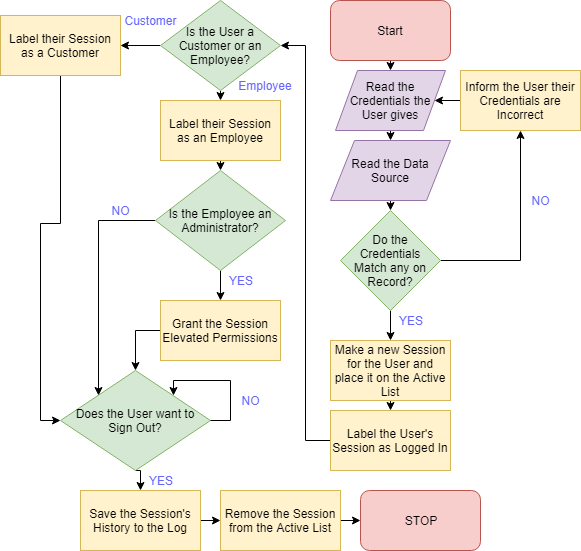
\includegraphics[width=\textwidth]{loginSystem.png}
    \centering
    \end{figure}
    \paragraph{•}
    A Session refers to the user's connection to the host computer; it is persistent while the user remains connected to the web application and can have many properties and pieces of data attached to it.
    The Active List is the conceptual area in memory where the hosting machine will keep track of all the currently active Sessions.
    \newpage
    \paragraph{Store Main Area}
    This page/area represents the forefront of the website as it is presented to the customer, and thus must be "slick" and comprehensive.
    According to my research, I have planned out filtering and sorting features within the page.
    \begin{figure}[h]
    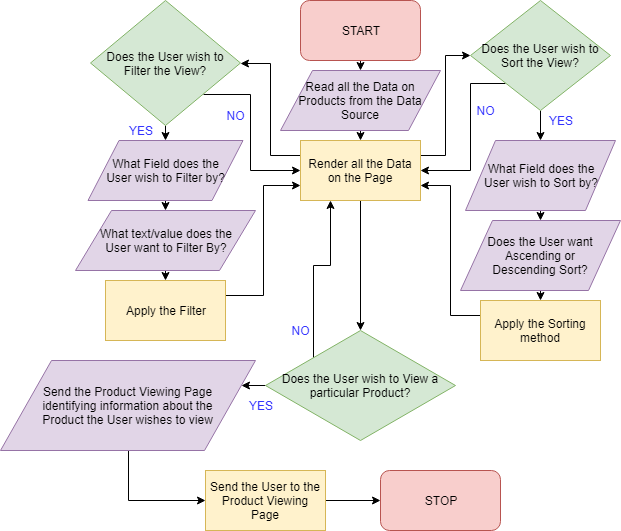
\includegraphics[width=\textwidth]{storefrontMain.png}
    \centering
    \end{figure}
    \paragraph{•}
    The algorithms used for sorting and filtering will be covered in more details in the algorithms section below.
    \newpage
    \paragraph{Product View Page}
    This page will be the "detailed" display of all the information regrading the product.
    It will show a set of images and a written, plain text description.
    Customers will be able to add a given amount of a product to their "cart" there.
    It is \textit{imperative} that the information displayed on this page is plentiful, and very legible.
    \begin{figure}[h]
    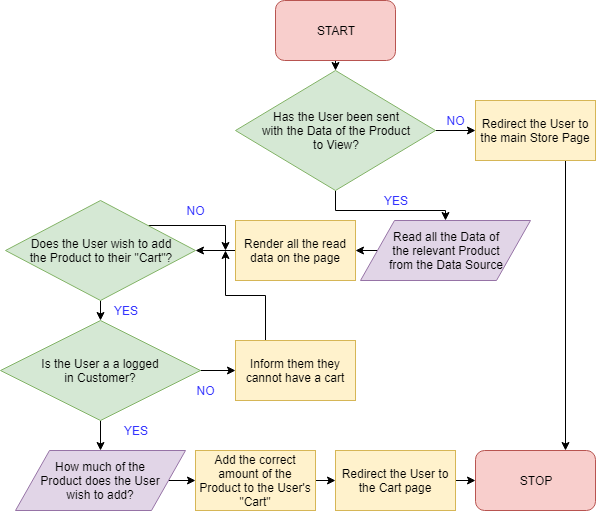
\includegraphics[width=\textwidth]{productPage.png}
    \centering
    \end{figure}
    \paragraph{•}
    The cart should be a collection of products stored in a group labelled with what customer has them in their cart.
    It should be independent of the Sessions so that customers can leave the website or sign out without losing the items in their cart.
    Users who aren't logged in to a customer account may not possess a cart because employees are not authorized to make purchases on the site and people who are not logged in at all may not possess a cart because an account is needed to make a purchase (so purchases are track able).
    \newpage
    \paragraph{Cart Page}
    The cart page shows the customer what they currently have in their cart, lets them edit amounts  and remove products.\\
    More importantly, this is the page where users will make their actual purchases from.
    There are several factors which should be considered in regard to this feature:
    \begin{itemize}
    \item Whether there is enough of all products in the inventory to supply the user's purchase
    \item The user's payment method
    \item The user's delivery address
    \end{itemize}
    After poring over these, I produced the following method.
    \begin{figure}[h]
    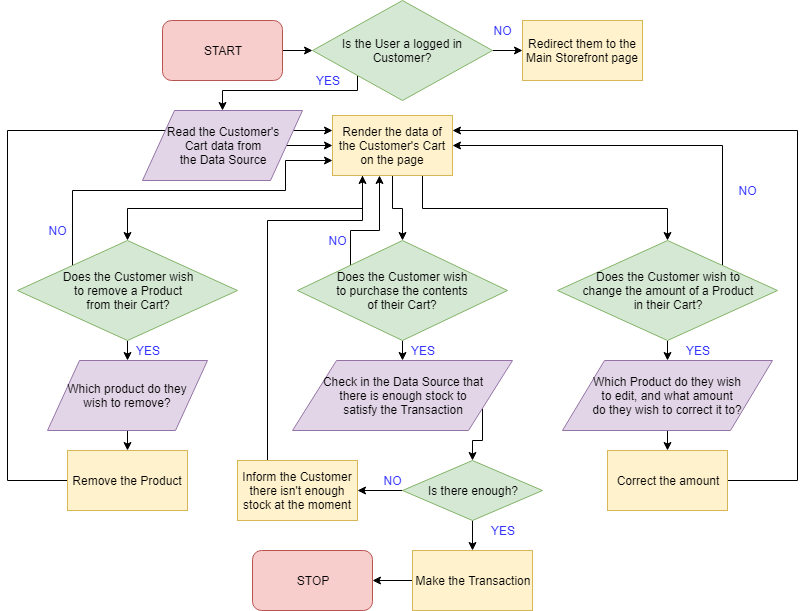
\includegraphics[width=\textwidth]{cartPage.png}
    \centering
    \end{figure}
    \paragraph{•}
    The transaction must be handled individually, as it's own process.
    While I cannot guess yet, managing monetary transactions may well prove to be out of the scope of this project, but this is yet to be proved.
    \newpage
    \paragraph{Physical Market Management Page}
    This page will be where the employee interacts with all features related to managing stock at third party events.
    Tt's appearance could quickly get confusing, so careful UI design is important.
    \begin{figure}[h]
    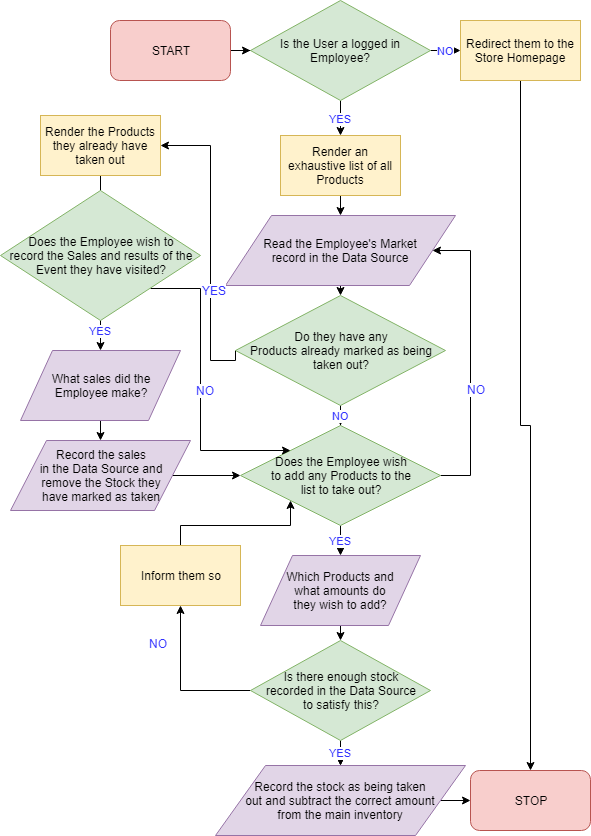
\includegraphics[scale=0.5]{physicalMarket.png}
    \centering
    \end{figure}
    \paragraph{}
    \newpage
    \subsection{Algorithms}  
    \paragraph{Quick Sort}
    One of the complex algorithms I will employ will be a sorting algorithm to sort lists of products to be displayed on the store front in good time.
    I chose the quick sort algorithm for this purpose because it is highly efficient across most datasets, having $O(log(n))$ average complexity and $O(n^2)$ worst case complexity, and because it offers the opportunity to be solved recursively.
    My pseudocode for the algorithm is as follows:
    \begin{lstlisting}
        function quicksort(dataset)
            switch input.length:
                case 1:
                    return dataset
                case 2:
                    if dataset[1] < dataset[0] then
                        dataset[0], dataset[1] = dataset[1], dataset[0]
                    endif
                    return dataset
            endswitch

            pivotindex = dataset.length / 2
            pivotindex = roundup(pivotindex)

            list under
            list over

            for i = 0 to (dataset.length - 1)
                if i == pivotindex then
                    continue
                elseif dataset[i] < dataset[pivotindex] then
                    under.add(dataset[i])
                elseif dataset[i] >= dataset[pivotindex] then
                    over.add(dataset[i])
                endif
            next i

            array underArray = quicksort(under.toarray())
            array overArray = quicksort(over.toarray())
            
            return underArray + dataset[pivotindex] + overArray
    \end{lstlisting}
    \subsection{Key Variables and Structures}
    \subsection{Usability Features}
    \subsection{Test Data}
    \newpage
    
    \section{Development}
    \subsection{Iterative Development}
    \subsection{Prototyping}
    \subsection{Annotated Code}
    \subsection{Validation}
    \subsection{Reviews}
    \newpage
    
    \section{Testing}
    \subsection{To Inform Development}
    \subsection{To Inform Evaluation}
    \newpage
    
    \section{Evaluation}
    \subsection{Testing}
    \subsection{Usability Features}
    \subsection{Evaluation}
    \subsection{Maintenance}
\end{document}
